\documentclass[11pt]{book}

\usepackage[width=7.0in, height=9.0in, top=1.0in, papersize={8.5in,11in}]{geometry}
\usepackage[pdftex]{graphicx}
%\usepackage{datetime}
\usepackage{anyfontsize}
\usepackage{t1enc}
\usepackage{verbatim}
\usepackage{algorithm}
\usepackage{algorithmic}
\usepackage{framed}
\usepackage{pdfpages}
\usepackage{listings}
\lstset{language=C}

\lstset{language=python,frame=ltrb,framesep=5pt,basicstyle=\normalsize,
 keywordstyle=\ttfamily\color{DarkRed},
%morecomment=[n][\textbf]{In\ [}{]\:},
%morecomment=[n][\textbf]{Out\ [}{]\:},
morecomment=[s][\color{blue}]{In\ [}{]\:},
morecomment=[s][\color{red}]{Out[}{]\:},
identifierstyle=\ttfamily\color{DarkBlue}\bfseries,
commentstyle=\color{DarkGreen},
stringstyle=\ttfamily,
showstringspaces=false,tabsize = 3}


\lstdefinelanguage{shell} {
commentstyle = \color{black},
keywordstyle = \color{black},
stringstyle = \color{black},
identifierstyle = \color{black},
morecomment=[s][\color{blue}]{In\ [}{]\:},
morecomment=[s][\color{red}]{Out[}{]\:},
 }

\pagestyle{empty}

\usepackage{helvet}
\renewcommand{\familydefault}{\sfdefault}

\begin{document}

\fontsize{16}{16}\selectfont Sprint Report \#2


\section{Team Members:}
Marcus Berger
\\Dicheng Wu\\
\textbf{Sponsor:}
\\Jeff McGough
\\

\section{Prototype Progress}
The progress is mostly out of the research phase and has began the first steps of production. The progress is laid out in more detail in this report. As of now the prototype is in a state to begin working on functionality. The rough (not final) GUI pages are laid out and being constructed to give us an environment for creating the functionality. The back end database has been constructed and will allow us to begin testing the database connected page as we create them. Current pages constructed are log in page, landing pages, and some options page.

\section{Project deliverables of Sprint 2:}

\begin{enumerate}
\item The database creation script  
\item Gui path work, meaning figuring out the path through the Gui
\item Log in page that reads users permission level and sends them to the correct landing page
\item Rough landing pages for Admin and Teachers (design improvements to come in later sprint) 
\end{enumerate}


\subsection{Sprint 2 Backlog:}

\begin{enumerate}
\item Creation of database tables 
\item Draw Gui path
\item Decision on rough Gui theme
\item Create a log in page that sends the user to the correct landing page based on their permission level
\item Create rough versions of teacher and admin landing pages to test functionally (improve look in latter sprint 
\item Continue rough gui page creation to have environments for functionality 
\item Sprint 2 Review
\item Continuing practice with QT
\end{enumerate}

\section{Database Creation}

The first thing we tackled in sprint 2 was getting the database up so we could begin actually developing the product and give our qt interface something to actually interface with. The main goal here was to make sure we had constructed the database in such a way that it could complete all the user stories it needed to in a way that made sense. After talking through the tables and the users stories we came up with the table creation script that was submitted with this sprint. While modifications will need to be made for when we do the billing side of the project, we think that this table structure should provide for the need of the academy.

A few thing to note in the database, we created student\_class and teacher\_class tables to deal with the many to many relationships in the database. Also there are no payroll or transaction tables yet as the group is still trying to figure out how to handle billing information and data.


\begin{figure}
\caption{Tables currently in database}
\centering
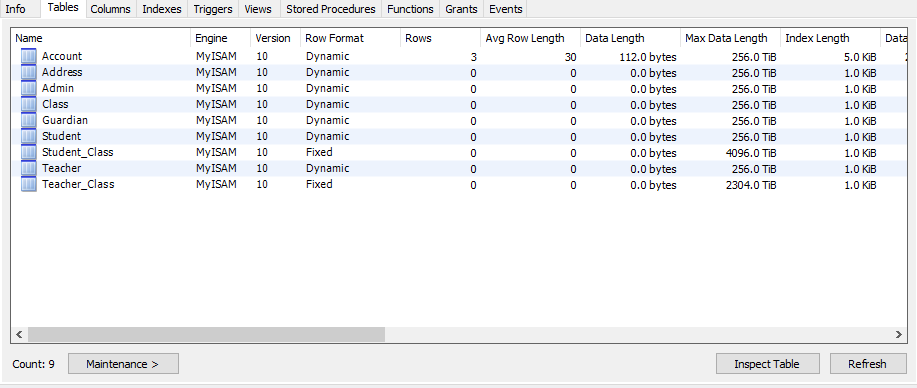
\includegraphics[width=0.5\textwidth]{database_tables}
\end{figure}

\section{GUI Work}

\subsection{GUI Path and Theme}

The path for the gui was part of the backlog so we could figure out the minimum number of pages we would need to do the things required by this project. This does not mean we are looking to create only the minimum but just get a general idea of how many pages we would need. Also it allowed us to see how the pages were connected and how we expect navigation through the system to work. The rough drawing of the path can be found in the Github repo's sprint two folder.

The other thing we need was to talk to the client about what he wanted for a navigation theme. We came up with three options, first was a button layout on the top and side of the page, second was  drop down menu similar to the way was mac and windows handle navigation in their products. Last was an expanding folder structure similar to that of the content management system Ektron. After consulting with Dr. Mcgough, he  decided that the more familiar drop down menu would be the easiest and most user friendly option and the option he would prefer we do. This decision allows us to use the built in menu bar functionality of pyqt and should reduce work load on navigation for this project.

Another part of theme is color and design, the color scheme will most likely resemble the academy's color plate, but the improve design will be worked on later. As of now the primary focus is making sure all the functionality works.


\subsection{GUI Pages}

The GUI pages for this sprint were the log in page and the landing pages for admin and teachers. The student part of the gui will be php which will be worked on in a future sprint once the functionlity is done. Since the student functions are similar to some of the admin or teacher functions most work should port over fairly quickly.

The first page we made was a login in page that takes a username and a password and first checks to see if they exist and are correct within the system. If they are not a dialog saying whats wrong appears and prompts the user again. If the information passes the check the system reads the users permission level and sends them to the corresponding landing page.

\begin{figure}
\caption{Current iteration of the log in page}
\centering
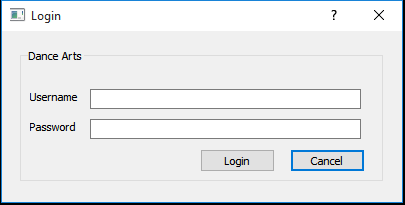
\includegraphics[width=0.5\textwidth]{login_page}
\end{figure}

The other set of pages we need to make to begin writing functionality was the landing pages for the admin and teacher permission levels. These pages show the types of things each can do and allow navigation to the various different functionality that permission level can do. For example the admin landing page has a button to take you to a student options page, from there you select which option you want and will be taken to the page to execute that function. The idea is to start at the landing page and be able to navigate to a specific function in three or four clicks max. The menu bar will also execute navigation and should allow the user to jump to a desired function.\\

\begin{figure}
\caption{Current iteration of the Admin Landing page}
\centering
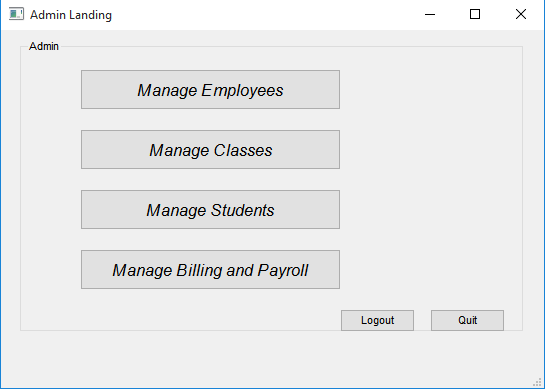
\includegraphics[width=0.5\textwidth]{admin_landing}
\end{figure}

Pages currently being worked on include:

\begin{enumerate}
\item Search pages
\item Modify data page
\item Add information and new information pages
\end{enumerate}


\section{Sprint 2 Issues}
Some issues that were encountered during this sprint were:

\begin{enumerate}
\item Running out of time - the group found it hard to complete this sprint on time due to many time draining issues, such as other class work,family matters, midterm exams and a client presentation during this sprint. Mitigation for this issue will be better time management for the team.
\item Inexperience with pyqt - The team ran into some issues that drained on time when working with pyqt, such as looking up information on how to perform a needed task. Mitigation for this issue is mostly experience based as we learn the system and learn how to more efficiently navigate the community the time sink should go down.
\item Team communication - The team found some issues in communicating with one another because of the language barriers within the team. Which in some cases slowed sprint progress. Mitigation for this issue will come with time as the group begin to understand each other better and find efficient patterns of communication.
\end{enumerate}

\section{Client Interactions}

Client interactions came in the form of weekly meeting every wednesday at 2:00 p.m. Topics included:

\begin{enumerate}
\item Progress reports on where we are in the project
\item Asking questions to refine functionality and understand academy needs
\item Discuss the future of the project and idea on how to execute them
\end{enumerate}


\section{Group Meeting}

The group has a standard meeting time of 4:00-5:00 or 4:00-6:00 MWF and a second meeting time of TTH 10:00 - 12:00

Meeting can continue pass these times if needed, and other times during the weekend. However weekend times fluctuate and do not remain constant from week to week. 

\section{Work Distribution}

Marcus:
\begin{enumerate}
\item Gui Path Charts
\item Landing page Construction\\
\end{enumerate}

Dicheng:
\begin{enumerate}
\item GUI Theme Ideas
\item Log In Page and Permission Navigation\\
\end{enumerate}


Together:
\begin{enumerate}
\item Wrote and talked through database and construction
\item Got database running
\item GUI page breakdown based on user stories and product backlog
\item Coded some functionality
\end{enumerate}

\end{document}